To validate our proposed algorithm we are providing numerical simulations in this chapter. First we solve the nonlinear PBE for the Krikwood sphere problem and compare the numerical results with the analytical solution. Then we consider a hypothetical protein molecule with just one atom for the PBE and solve it to compare with the analytical result. 

%%%%%%%%%%%%%%%%%%%%%%%%%%%%%%%%%%%%%%%%%%%%%%%%%%%%%%%%%%%%%%%%%%%%%%%%%%%%%

\section{Krikwood Sphere with analytical solution}
\label{krik}

The analytical solutions of the PBE are available only for simple geometries such as spheres. We have chosen the benchmark problem known as the Krikwood sphere, where a sphere has a charge at its center. This problem has the following analytical solution  (\ref{eq:sphere1}) with the source term (\ref{eq:sphere2}) as described in \cite{Geng2013_Fully}. 
\begin{align}
	\phi({\bf r})&=\left\{\begin{array}{lc}\displaystyle\frac{1}{\varepsilon R}-\frac{1}{R}+\displaystyle\frac{1}{||{\bf r}||} & ||{\bf r}||<R, \\
	\displaystyle\frac{1}{\varepsilon ||{\bf r}||}& ||{\bf r}||>R.\end{array}\right.\label{eq:sphere1}\\
	\rho({\bf r})&=\left\{\begin{array}{lc}4\pi \delta ({\bf r)} & ||{\bf r}||<R, \\ \displaystyle\bar{\kappa}^2\sinh (\frac{1}{\varepsilon ||{\bf r}||}) & ||{\bf r}||>R,\end{array}\right.\label{eq:sphere2}
\end{align}
where $\varepsilon=\epsilon^+ / \epsilon^-$ and $R=2$ is the radius of the sphere and $\bar{\kappa}=1$. We have a unit charge $1e_c$ located at the center of the sphere $(0,0,0)$. Altogether this sphere is comparable to a protein molecule located inside our computational domain set by the boundaries form $-7$ to $7$ in $x,y$ and $z$ directions.  Here the dielectric constants are set as $\epsilon^+=80$ outside the sphere and $\epsilon^-=1$ inside the sphere. The ionic strength is $I_s = 0.01$ for all the tests discussed in this Section for the Krikwood sphere problem. It can be shown that this analytical solution in (\ref{eq:sphere1}) with the source term defined in (\ref{eq:sphere2}) will satisfy the nonlinear PBE in (\ref{pbe}) together with the jump condition defined in (\ref{ju_cond}). Both of the major challenges like the singularity and the non-smoothness are present in this benchmark problem. For an example the singularity is generating from the source term in (\ref{eq:sphere2}) for $||{\bf r}|| <R$. Also the non-smoothness is present due to the jump condition (\ref{ju_cond}). Both of these difficulties gives similar kind of challenge present in the nonlinear PBE to reduce the accuracy of the spatial discretization numerically. To use this benchmark problem to test the stability and the convergence in time and space we computed the $L_2$ error and $L_\infty$ error using the following measures: 
\begin{equation}
	L_\infty=\max\limits_{i,j,k}|\phi_{\rm exact}-\phi_{\rm num}|, L_2 = \sqrt{\frac{\sum_{i,j,k}|\phi_{\rm exact}-\phi_{\rm num}|^2}{N}},\label{eq:l2lmax}
\end{equation}
where $\phi_{\rm true}$ is the analytical solution and $\phi_{\rm num}$ is the numerical solution representing the electrostatic potential for the nonlinear PBE. For the $L_2$ error we have used $N= N_x \times N_y \times N_z$ as the total number of unknowns on the grid points. 
\begin{figure}[!ht]
	\centering
	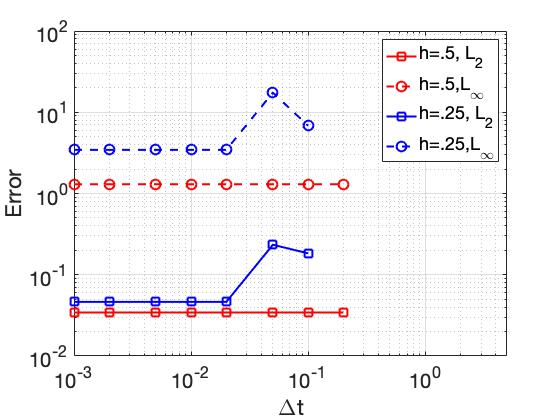
\includegraphics[width = 3in]{stab_adi.jpg}
	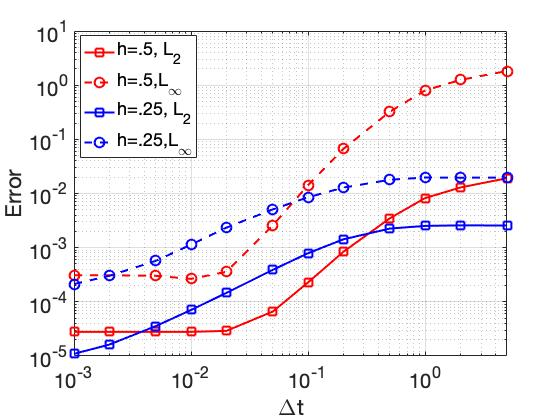
\includegraphics[width = 3in]{stab_gfmadi.jpg}\\
	(a)ADI\hspace*{2.5in} (b)GFM-ADI\\ 	
	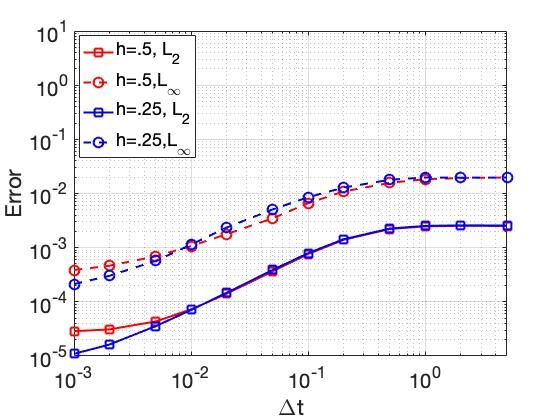
\includegraphics[width = 3in]{stab_gfmlodcn.jpg}
	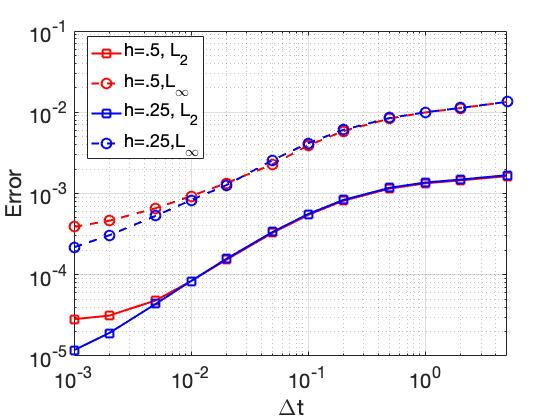
\includegraphics[width = 3in]{stab_gfmlodie.jpg}\\
	(c)GFM-LODCN \hspace*{2in} (d)GFM-LODIE
	\caption{Stability test for the Krikwood Sphere with $T_{end}= 10^4*\Delta t$.}
	\label{fig:stab_krik}	
\end{figure}

\textbf{Stability Test:} One way to test the stability of the numerical methods used to solve the PBE is to run the time loops for a lot of iterations to check if they diverge or blow-up. In this study we chose to run the whole process for $10^4$ iterations for different choices of time step size $\Delta t$ for each one of our proposed  methods along with the previous ADI method \cite{Geng2013_Fully}. Our goal here is to check if these numerical methods are unconditionally stable or not for different choices of $\Delta t$ and if they are conditionally stable then what is the condition on the best choice for $\Delta t$. We focused on the variation of only $\Delta t$ and used finer grids such as $h = 0.5$ and $h = 0.25$ to avoid the difficulty due to the larger grid spacing. We have found all three of our methods to be stable for $\Delta t \in [0.001,5]$ for this benchmark problem. To illustrate this we considered the sampling for $\Delta t $ such as $\Delta t \in t_{set}=\{0.001, 0.002, 0.005,0.01, 0.02, 0.05, 0.1, 0.2, 0.5, 1,2,5\}$ and the stopping time $T_{end}= 10^4*\Delta t$, so that enough accumulations of numerical errors are experienced. 

We observe in Figure \ref{fig:stab_krik} (b), (c) and (d) that both $L_2$ and $L_\infty$ errors to be finite for all $\Delta t \in t_{set}$. For larger values of $\Delta t$ such as $\Delta t =5$, the numerical errors might feel meaningless but as long as these errors remain finite, this demonstrates the stability of the underlying time integration.  In comparison the ADI method \cite{Geng2013_Fully} in Figure \ref{fig:stab_krik} (a), blows-up for $\Delta t > 0.2$ in both cases. Also the error lines are almost flat (constant) for $\Delta t <0.02$ in Figure \ref{fig:stab_krik} (a), indicating that the $L_2$ and $L_\infty$ error are polluted and dominated by the singularities at the center of the sphere and do not decrease when $\Delta t$ becomes smaller like the other methods do. This observation again emphasizes the importance of regularization to avoid the singularity of the PBE. 


\begin{table}[!ht]
\centering
%\begin{tabular}{|c|c|c|c|c|c|}
\begin{tabular}{c c c c c c }
\hline
$h$ & $L_2$ & Order & $L_\infty$& Order & $E_{\rm sol}$ \\ \hline
\multicolumn{6}{c}{ADI} \\ \hline
  2 & 6.45E-03 & N/A & 3.82E-02 & N/A & -92.699927 \\ %\hline
  1 & 4.88E-03 & 0.40 & 7.61E-02 & -0.99& -83.683388 \\% \hline
1/2 & 3.43E-02 & -2.81 & 1.30E+00 & -4.09 & -85.921222 \\ %\hline
1/4 & 4.63E-02 & -0.43 & 3.44E+00 & -1.41 & -83.279725 \\ %\hline
1/8 & 5.11E-02 & -0.14 & 7.49E+00 & -1.12 & -82.680633 \\ \hline

%\multicolumn{6}{|c|}{GFM-ADI} \\ \hline
\multicolumn{6}{c}{GFM-ADI} \\ \hline
  2 & 3.14E-04 & N/A & 1.82E-03 & N/A & -81.742795 \\ %\hline
  1 & 1.18E-04 & 1.41 & 8.28E-04 & 1.13 & -82.132181 \\% \hline
1/2 & 2.79E-05 & 2.08 & 3.10E-04 & 1.42 & -82.063724 \\ %\hline
1/4 & 8.51E-06 & 1.71 & 1.23E-04 & 1.34 & -82.051117 \\ %\hline
1/8 & 1.49E-06 & 2.51 & 4.47E-05 & 1.46 & -82.046462 \\ \hline
%\multicolumn{6}{|c|}{GFM-LODCN} \\ \hline
\multicolumn{6}{c}{GFM-LODCN} \\ \hline
%h & $L_2$ & Order & $L_\infty$& Order & $E_{\rm sol}$ \\ \hline
  2 & 3.14E-04 & N/A  & 1.82E-03 & N/A  & -81.742788 \\ %\hline
  1 & 1.18E-04 & 1.41 & 8.89E-04 & 1.03 & -82.132148 \\ %\hline
1/2 & 2.87E-05 & 2.04 & 3.87E-04 & 1.20 & -82.063684 \\ %\hline
1/4 & 1.10E-05 & 1.39 & 2.13E-04 & 0.86 & -82.051064 \\ %\hline
1/8 & 7.16E-06 & 0.62 & 1.41E-04 & 0.60 & -82.046402 \\ \hline
%\multicolumn{6}{|c|}{GFM-LODIE} \\ \hline
\multicolumn{6}{c}{GFM-LODIE} \\ \hline
%h & $L_2$ & Order & $L_\infty$& Order & $E_{\rm sol}$ \\ \hline
2   & 3.16E-04 & N/A   & 1.84E-03 & N/A   & -81.738399 \\ %\hline
1   & 1.17E-04 & 1.43  & 8.85E-04 & 1.06  & -82.123319 \\ %\hline
1/2 & 2.84E-05 & 2.05  & 3.89E-04 & 1.19  & -82.055388 \\ %\hline
1/4 & 1.18E-05 & 1.27  & 2.18E-04 & 0.83  & -82.043011 \\ %\hline
1/8 & 9.40E-06 & 0.33  & 1.48E-04 & 0.56  & -82.046402 \\ \hline
\end{tabular}
\caption{Spatial Convergence test for the krikwood sphere with $\Delta t = 0.001$ and $T_{end}=10$. Comparable analytical value of the Solvation Energy is $E_{sol} = -81.97820845$.}
\label{tab:krikwood}
\end{table}


\textbf{Spatial Convergence:}  In this study, we investigated the order of accuracy for the spacial convergence in terms of $L_2$ and $L_\infty$ error using equation (\ref{eq:l2lmax}) in Table \ref{tab:krikwood} for the Krikwood sphere. The time step size $\Delta t$ is kept fixed at $\Delta t = 0.001$ while the grid spacing $h$ is reduced from $2$ to $1/8$. Within this range of $h$ we have noticed the accuracy of the GFM-ADI to be nearly 2nd order while it gradually decreases for the GFM-LODCN and GFM-LODIE. In this experiment, the stopping time has been set to $T_{end} = 10$ and found to be long enough to produce acceptable results. We have also computed the solvation energy $E_{\rm sol}$ for the nonlinear PBE in (\ref{pbe}) with the source term defined in (\ref{rho}). The solvation energy for this setup can also be computed analytically as $-81.97820845$. For all three of our proposed methods the solvation energies $E_{\rm sol}$ are found to be very close to this analytical value as reported in Table \ref{tab:krikwood}. In comparison the accuracy of the ADI method decreases instead of increasing as the grid spacing becomes finer. The major reason behind this is the singularity at the center being one of the grid points. The actual difference between the numerical solution and the analytical solution is $\infty$ since the term $\displaystyle \frac{1}{||{\bf r}||} $ in the analytical solution becomes $\infty$ at the center of the sphere. So we avoided this point to calculate our $L_2$ and $L_\infty$ errors  showed in Table \ref{tab:krikwood}. But still, it affects the neighboring points error and ultimately dominates the errors at all other points.    

\begin{figure}[!ht]
	\centering
%	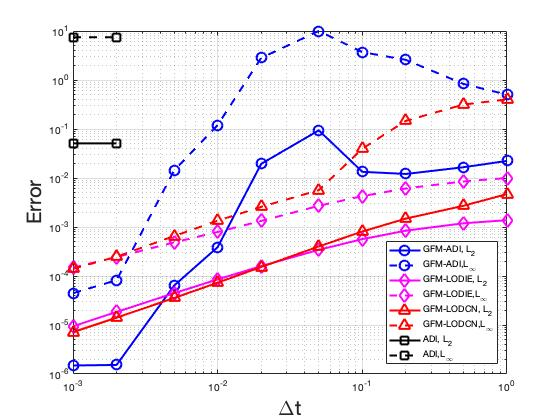
\includegraphics[width=4in]{temp.jpg}
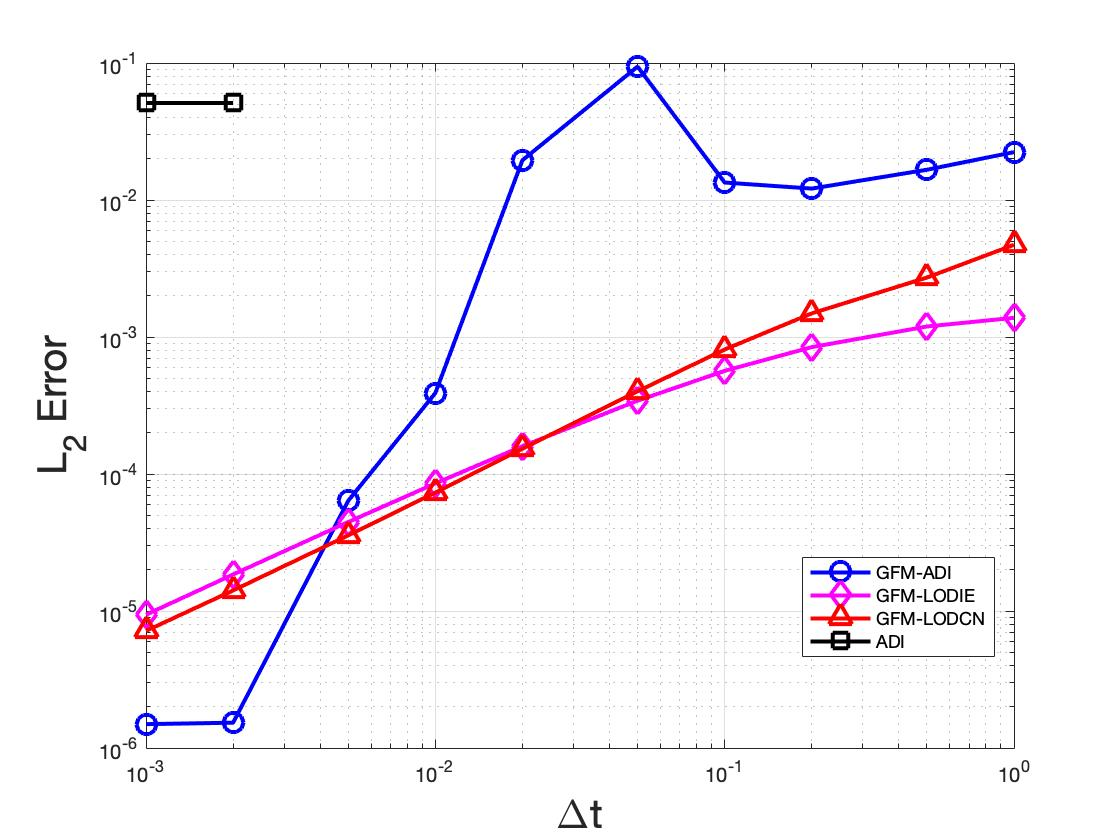
\includegraphics[width=3in]{temp_1.jpg}
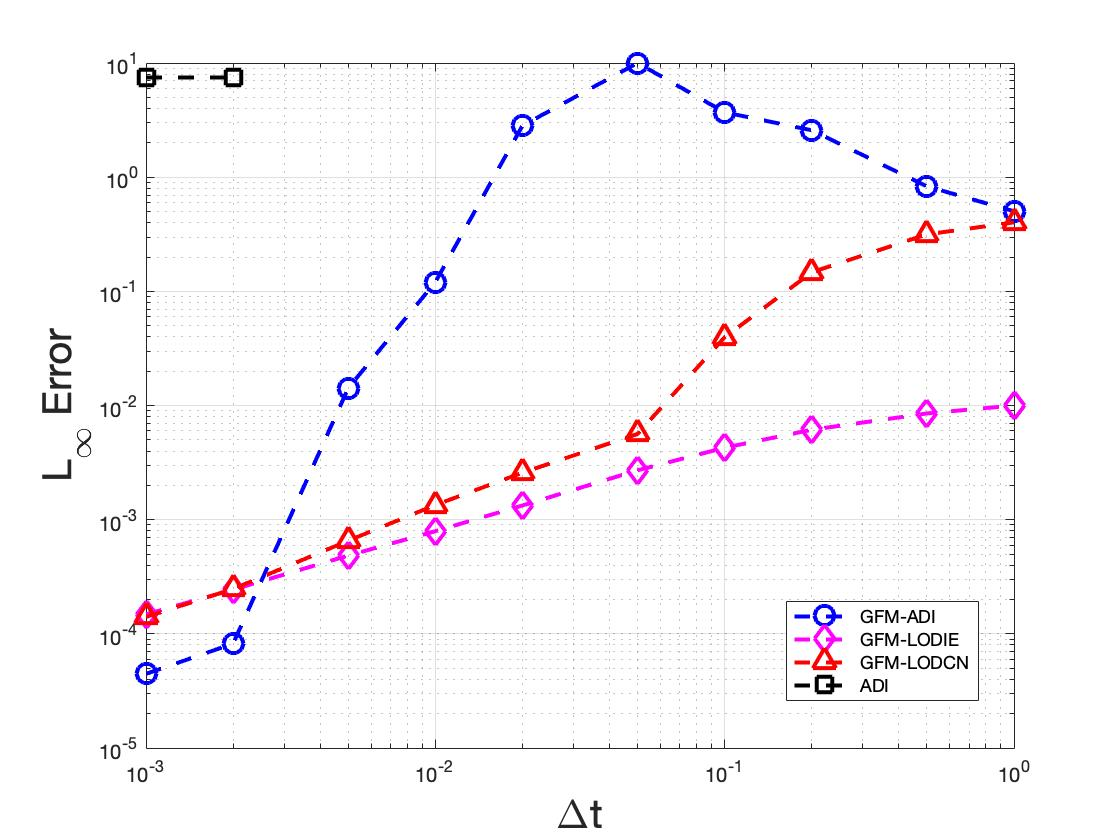
\includegraphics[width=3in]{temp_2.jpg}
   (a)\hspace*{3in} (b)\\ 	
	\caption{Temporal Convergence test for the krikwood sphere with $h=0.125$ and $T_{end} = 10$.}
	\label{fig:temp_Krik}
% Datas for Tend = 100 is available in RC2 c.  	
\end{figure}

\textbf{Temporal Convergence:} Finally we investigate the temporal convergence of all three of our proposed methods for the Krikwood Sphere in Figure \ref{fig:temp_Krik} along with the ADI method. Similar to the spatial convergence test we have chosen the fixed stopping time to be $T_{end} = 10$ and $\Delta t \in \{0.001, 0.002, 0.005,0.01, 0.02, 0.05, 0.1, 0.2, 0.5, 1\}$. As we observe in Figure \ref{fig:temp_Krik}, GFM-ADI is the most accurate method for the smaller $\Delta t$ but as $\Delta t$ increases GFM-LODCN and GFM-LODIE perform better than GFM-ADI in terms of both the $L_2$ and $L_\infty$ errors. For the larger $\Delta t $ GFM-LODIE method remains the most accurate. In comparison the ADI method represented by the black lines in Figure \ref{fig:temp_Krik} blows-up just after $\Delta t = 0.002$. This indicates that we can choose larger time step sizes $\Delta t$ for the newly proposed methods compared to ADI method which will eventually require less time to reach the steady state solution.   


%%%%%%%%%%%%%%%%%%%%%%%%%%%%%%%%%%%%%%%%%%%%%%%%%%%%%%%%%%%%%%%%%%%%%%%%%%%%%
   
\section{Biological applications}

In this section, we focus on exploring the stability and accuracy of GFM-ADI, GFM-LODCN and GFM-LODIE schemes by considering the solvation analysis of proteins. Even though all of our proposed schemes were found to be stable for the one atom case (Krikwood sphere) with $\Delta t =[0.001,5]$, it is of great interest to see if these schemes are stable for real protein systems. We will compare all three methods in detail for a particular protein system and try to identify the best choice for the time increment $\Delta t $ and the grid spacing $h$ to get the most accurate result within a reasonable amount of time. The optimum $\Delta t$ and $h$ are used later to calculate the solvation energy of 24 proteins.      
%%%%%%%%%%%%%%%%%%%%%%%%%%%%%%%%%%%%%%%%%%%%%%%%%%%%%%%%%%%%%%%%%%%%%%%%%%%%%

\subsection{Protein Crambin } To validate our proposed schemes with a real protein we consider the hydrophobic protein Crambin (PDB ID : 1cbn). It is a 46 residue protein homologous to a membrane-active plant toxins \cite{1cbn_paper}. It is found in the seeds of \textit{Crambe abyssinicia} and has local anesthetic activity in a lobster leg axon (J. Marquis \cite{1cbn_paper}). We used the MSMS package to generate the molecular surface for this protein using the crystallographic data recored at $130 K$ as reported in \cite{1cbn_paper}. For this step we use the probe radius of $1.4$ and the density of $10$ in the MSMS package to calculate the molecular surface.

  In this study at first we report the solvation energy of 1cbn calculated by all three of our proposed schemes in Table \ref{tab-1cbn}. After calculating the electrostatic potential $\phi$, equation (\ref{eq:solvation}) is discretized further to calculate the solvation energy using equation (\ref{eq:solvation}) where $Q$ is the trilinear interpolation of the singular charges $q_i$ at the center of the atoms.  The potential values are obtained by scaling our calculated dimensionless potentials with the constant $0.596163438$ corresponding for the room temperature (300K). In all cases a uniform mesh size $h = 0.5$ and a large stopping time $T_{end}$ are used to ensure that the steady state solution is reached. For the dielectric constant we have used $\epsilon^+=80$ for water as the solvent and $\epsilon^-=1$ the region in side the protein. The ionic strength is set to $I_s = 0.15$.
% Table generated by Excel2LaTeX from sheet '1cbn'
\begin{table}[!ht]
\centering
\begin{tabular}{c c c c c }
\hline
%      & \multicolumn{3}{c }{h =1/2}                   \\ \hline
$\Delta t$  & ADI  & GFM-ADI       & GFM-LODCN     & GFM-LODIE     \\ \hline
%0.001 & -302.90138868 & -302.83729044 & -302.03341621 \\ %\hline
%0.005 & -302.90138868 & -302.83729044 & -302.03341621 \\ %\hline
%0.01  & -302.85075766 & -302.68957418 & -301.31096348 \\ %\hline
%0.02  & -302.69227062 & -302.33466174 & -300.06953533 \\ %\hline
%%0.03  & -302.49342491 & -301.93879794 & -298.97743897 \\ \hline
%%0.04  & -302.27488337 & -301.51872505 & -297.97906854 \\ \hline
%0.05  & -302.04538862 & -301.08386563 & -297.04896758 \\ %\hline
%%0.06  & -301.80951214 & -300.64096822 & -296.17267652 \\ \hline
%%0.07  & -301.56994437 & -300.19496277 & -295.34086258 \\ \hline
%%0.08  & -301.32859818 & -299.74929181 & -294.54698251 \\ \hline
%%0.09  & -301.08701698 & -299.30637260 & -293.78618610 \\ \hline
%0.1   & -300.84648128 & -298.86787256 & -293.05472908 \\ %\hline
%0.2   & -298.63624081 & -294.81110682 & -286.88648904 \\ %\hline
%%0.3   & -296.77150162 & -291.23283125 & -282.05981018 \\ \hline
%0.5   & -293.21633440 & -284.83429816 & -274.64462149 \\ %\hline
%0.7   & NaN           & -279.04495504 & -269.01031327 \\ %\hline
%%0.9   & NaN           & -273.75954410 & -264.47533078 \\ \hline
%1     & NaN           & -271.29161057 & -262.50478312 \\ %\hline
%2     & NaN           & -251.54655749 & -248.89416804 \\ %\hline
%%3     & NaN           & -237.49060662 & -240.78175990 \\ \hline
%5     & NaN           & -218.29937773 & -230.91124478 \\\hline
0.001 & -459.5742719854 & -303.00657886  & -303.00154088   & -302.80556740 \\
0.002 & -458.1104685049 & -302.99808443  & -302.98279503   & -302.61375402 \\
0.005 & -452.1116748705 & -302.90138868  & -302.83729044   & -302.03341621   \\
0.01  &    NaN         & -302.85075766   & -302.68957418   & -301.31096348   \\
0.02  &    NaN         & -302.69227062   & -302.33466174   & -300.06953533   \\
0.05  &    NaN          & -302.04538862   & -301.08386563   & -297.04896758   \\
0.1   &    NaN          & -300.84648128   & -298.86787256   & -293.05472908   \\
0.2   &    NaN           & -298.63624081   & -294.81110682   & -286.88648904   \\
0.5   &    NaN          & -293.21633440   & -284.83429816   & -274.64462149   \\
0.7   &   NaN           & NaN             & -279.04495504   & -269.01031327   \\
1     &     NaN         & NaN             & -271.29161057   & -262.50478312   \\
2     &    NaN          & NaN             & -251.54655749   & -248.89416804   \\
5     &    NaN           & NaN             & -218.29937773   & -230.91124478 \\ \hline
\end{tabular}
\caption{Stability test for the calculation of the Solvation Energy ({\it kcal/mol}) of 1cbn for $h=0.5$, $T_{end} = 10^4*\Delta t$.}
\label{tab-1cbn}
\end{table}

{\bf Stability Analysis:} Here we try to identify the value of $\Delta t$ as large as possible without losing too much accuracy for a real protein like 1cbn. Note that in Table \ref{tab-1cbn} for $\Delta t > 0.5$, the GFM-ADI diverges while the other two schemes lose significant amount of accuracy. If we consider the solvation energy ($\approx $ -302 {\it kcal/mol}) for $\Delta t =0.005$ to be accurate enough and compare all other solvation energies in Table \ref{tab-1cbn}, it can be observed that with the increase of $\Delta t$ in all three proposed schemes lose accuracy but at a different rate. The GFM-ADI scheme is usually more accurate while GFM-LODIE scheme is more robust it remains stable for larger values of $\Delta t$. The performance of the GFM-LODCN is roughly in between the other two schemes in terms of accuracy and stability. To be uniform  among all three proposed methods and the other proteins in this dissertation we have used the optimum value for $\Delta t =0.05$ and $h=0.5$. To chose the optimum value of $\Delta t$ and $h$ we consider the highest possible value for all three methods without loosing the accuracy too much. For the GFM-ADI method, the critical value of $\Delta t$ (in this case $0.5$) for stability gives us a safe zone ($\Delta t < 0.5$). Within this safe zone, the GFM-ADI method is both accurate and efficient. In comparison, for the ADI method this critical value is $\Delta t = 0.005$ which results in taking unreasonably longer time to reach the steady state to produce any results. 

Altogether GFM-ADI method is much more stable than the ADI method. This makes GFM-ADI a very practical method, while the ADI method is impractical by requiring too small $\Delta t$ values. In some sense, the GFM-ADI method is even better than LOD methods. Although LOD methods are unconditionally stable, the energies are inaccurate for large $\Delta t$ values. For GFM-ADI, the critical $\Delta t$ value for stability tells us a safe zone, within this safe zone, the GFM-ADI is both accurate and efficient. 

\begin{figure}[!ht]
	\begin{center}
	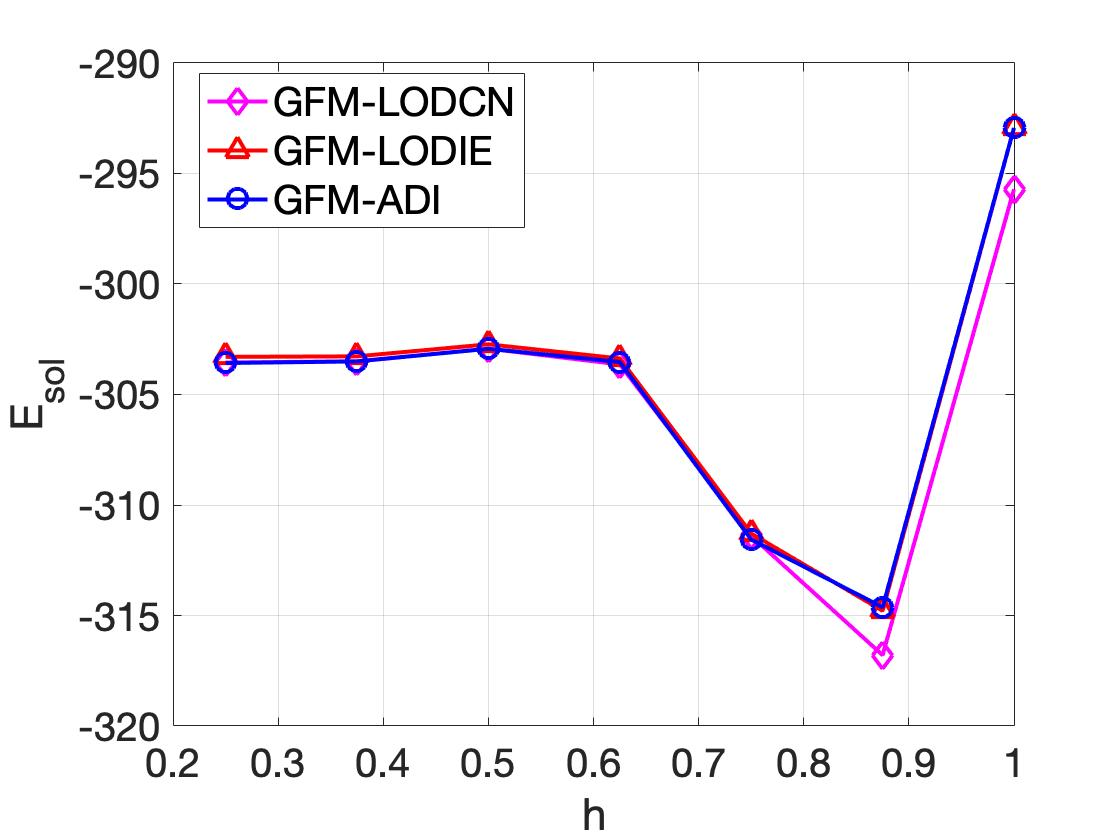
\includegraphics[width=3in]{space_1cbn_sol.jpg}
	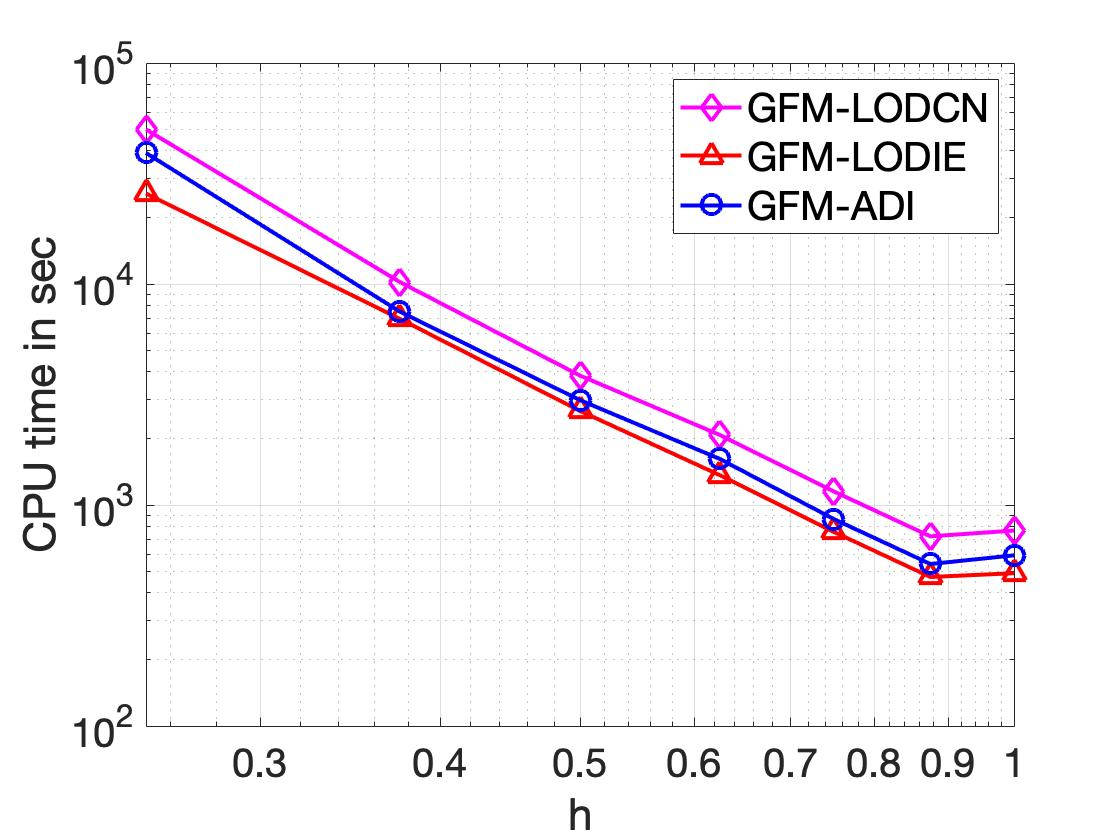
\includegraphics[width=3in]{space_1cbn_cpu.jpg}	
	(a)\hspace*{3in} (b)\\ 
	\end{center}
	\caption{Spatial convergence for \textit{1cbn} with $\Delta t = 0.001$ and $T_{end} = 10$.}
	\label{fig:space_1cbn}
\end{figure}

{\bf Spatial Convergence:} In Figure \ref{fig:space_1cbn} we investigate how the change of grid spacing $h$ affects the solvation energy of real proteins like $1cbn$. We keep the time increment small and fixed to $ \Delta t = 0.001$ with the stopping time $T_{end} = 10$. From Figure \ref{fig:space_1cbn} (b) it is clear that the required CPU time increases dramatically when the grid spacing $h$ decreases. So we need to find the value of $h$ as large as possible without losing too much accuracy. We also observe in Figure \ref{fig:space_1cbn} (a) that for $h<0.6$ the solvation energy doesn't change that much indicating that $h = 0.5$ might be the optimum choice for the calculation of the solvation energy of proteins. 

\begin{figure}[!h]
	\centering
	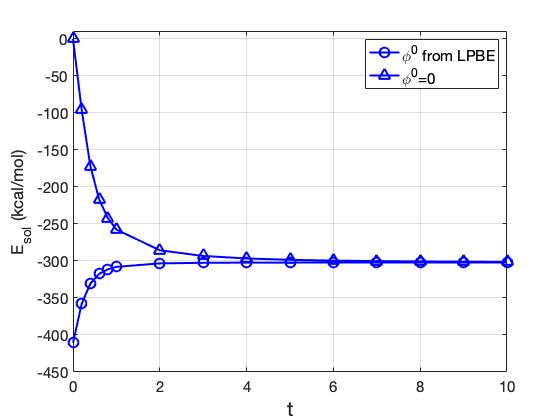
\includegraphics[width=0.49 \textwidth ]{tend_5.jpg}
	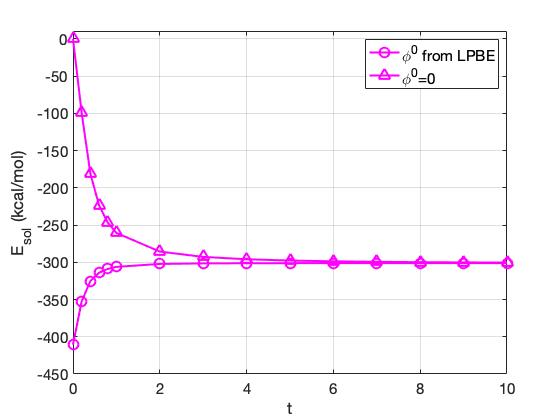
\includegraphics[width=0.49 \textwidth ]{tend_6.jpg}\\
	(a)\hspace*{3in} (b)\\ 
	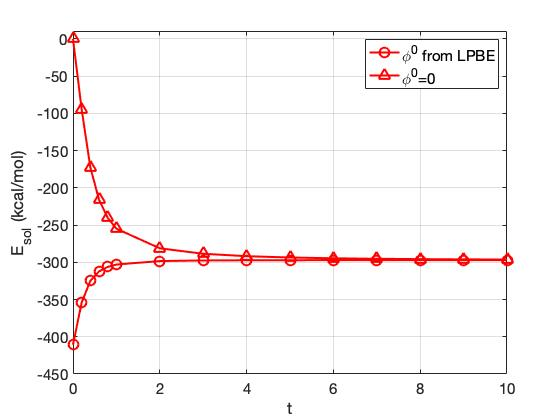
\includegraphics[width=0.49 \textwidth ]{tend_7.jpg}
	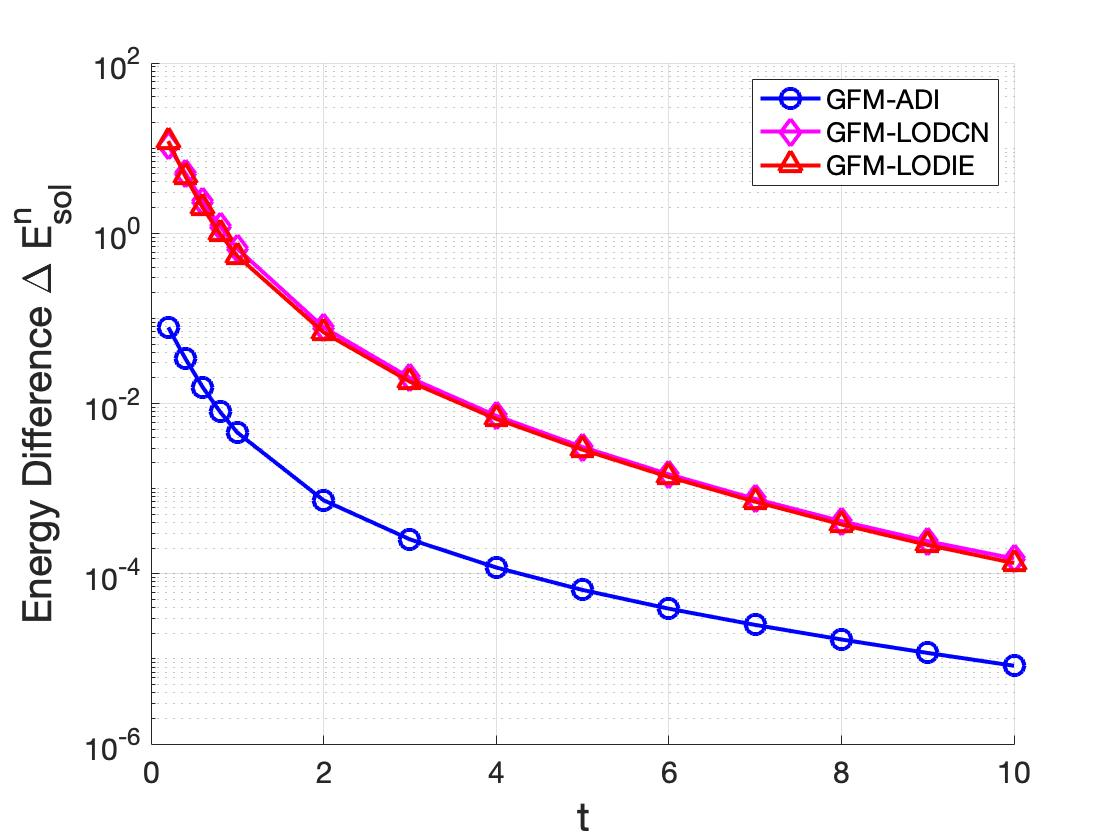
\includegraphics[width=0.49 \textwidth ]{tend_rel.jpg}
	(c)\hspace*{3in} (d)
	\caption{Steady State Analysis: The Solvation Energy (\textit{kcal/mol}) of $1cbn$ with $h=0.5$, $\Delta t = 0.05$ as $t\rightarrow \infty$. (a) GFM-ADI, (b) GFM-LODCN, (c) GFM-LODIE, (d) Solvation Energy difference  $\Delta E^n_{sol}(\phi^n)$.}
	\label{fig:tend}
\end{figure}

{\bf Steady State (as $t\rightarrow \infty$):} The pseudo-transient methods proposed in this dissertation usually approaches a steady state as $t\rightarrow \infty$. But with a nonlinear operator there is always a question wheather the steady state solution is unique or not. 
%Once the electrostatic potential $\phi^n$ achieves the steady state, further calculations are redundant. Hence identifying the time when $\phi$ arrives at the steady state and setting it as the stopping time $T_{end}$ is very important. 
Hence, we have tried two different type of initial condition to check if the proposed methods reach to the same steady state solution. For the fist type, we just set $\phi^0=0$. Then for the second type we solve a linearized PBE (LPBE) \cite{Zhao2011} and use the solution to initialize $\phi^n$ as $\phi^0 = $ "the solution of the LPBE". We fix the grid spacing $h = 0.5$ and the time step $\Delta t = 0.05$ and run the iterations until $t = 10$.
As we can see in Figure \ref{fig:tend} (a), (b) and (c), all of our proposed methods reach the same steady state solution for both type of initial condition demonstrating its uniqueness. It is also noticeable in Figure \ref{fig:tend} (a), (b) and (c), that initializing $\phi^n$ from LPBE is better than initializing $\phi^n$ as zero since it reaches the steady state earlier.     
  In Figure \ref{fig:tend}(d) we report the calculated solvation energy difference $\Delta E^n_{sol}$ at the n-th time step defined as,
\begin{equation}
	\Delta E^n_{sol}(\phi^n)= |E^n_{sol}(\phi^n)-E^{n-1}_{sol}(\phi^{n-1})|.
\end{equation}
As we observe in Figure \ref{fig:tend}(b), this energy difference $\Delta E^n_{sol}$ decreases over time and it can be another tool to identify the steady state set stopping time $T_{end}$.
\begin{table}[!ht]
\begin{center}
\begin{tabular}{c c c c }
\hline
X            & Y            & Z            & $E_{sol}$    \\ \hline
{[}-10,32{]} & {[}-9,29{]}  & {[}-15,28{]} & -302.0594 \\ \hline
{[}-13,35{]} & {[}-12,32{]} & {[}-18,31{]} & -302.0594\\ \hline
{[}-16,38{]} & {[}-14,35{]} & {[}-20,34{]} & -302.0626 \\ \hline
{[}-19,41{]} & {[}-17,38{]} & {[}-23,36{]} & -302.0656\\ \hline
\end{tabular}
\end{center}
\caption{Impact of domain size to the solvation energy of $1cbn$ calculated by the GFM-ADI method.}
\label{tab:domain}
\end{table}

Finally we investigate the effect of the size of the computational domain on the calculation of the solvation energy. As we observe in Table \ref{tab:domain}, changing the length of the cuboidal domain in the $x,y$ and $z$ directions up to $18$\r{A} doesn't change the solvation energy for $1cbn$ significantly. So we set the computational domain as small as possible keeping the whole molecule inside plus a fixed distance from the furthest atom from the coordinate origin.   


{\bf Electrostatic potential on the molecular surface:} In Figure \ref{fig_1cbn} we focus on the electrostatic potential on the surface of the protein 1cbn for all three of our proposed schemes. The difference is not that much noticeable unless we focus in the black squared region of the front side. This shows that even though there are some differences in the solvation energies calculated by the proposed three methods there is no significant difference for the electrostatic potentials for our choice for the optimum values of the parameters.    

\begin{figure}[!ht]
\begin{center}	
	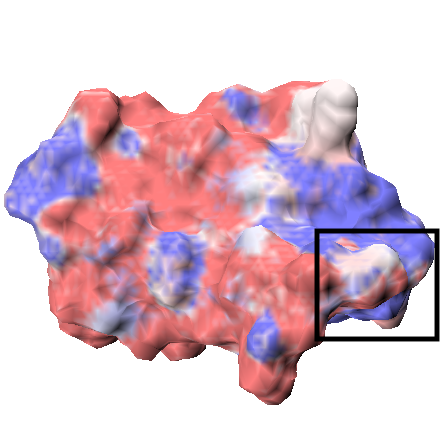
\includegraphics[width=2.1in]{1cbn_gfmadi_front_sq.png}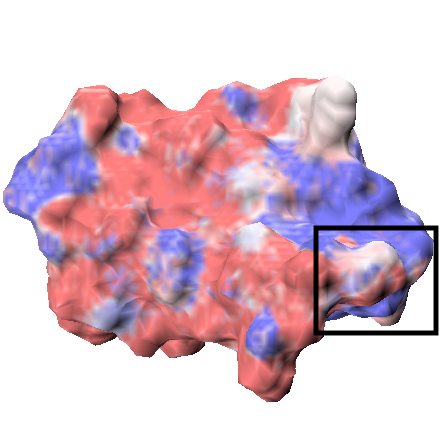
\includegraphics[width=2.1in]{1cbn_gfmlodcn_front_sq.png}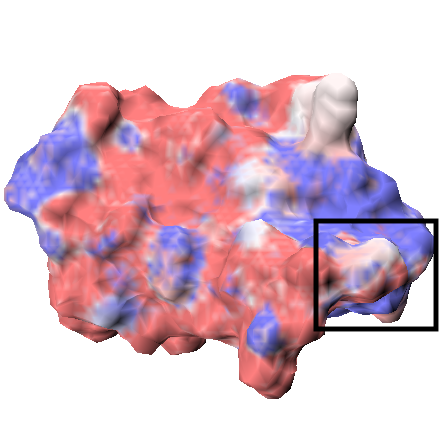
\includegraphics[width=2.1in]{1cbn_gfmlodie_front_sq.png}\\
GFM-ADI front \hskip 0.7in GFM-LODCN front \hskip 0.7in GFM-LODIE front\\
	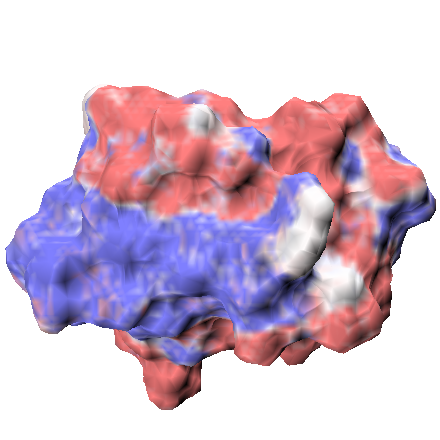
\includegraphics[width=2.1in]{1cbn_gfmlodcn_back.png}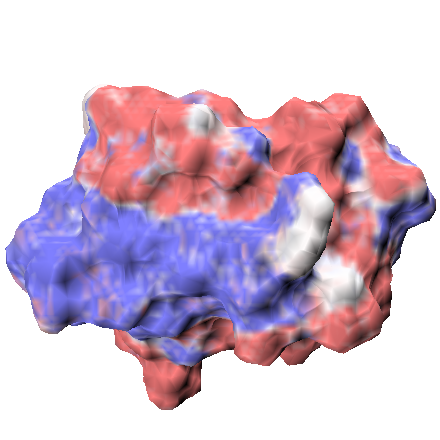
\includegraphics[width=2.1in]{1cbn_gfmlodcn_back.png}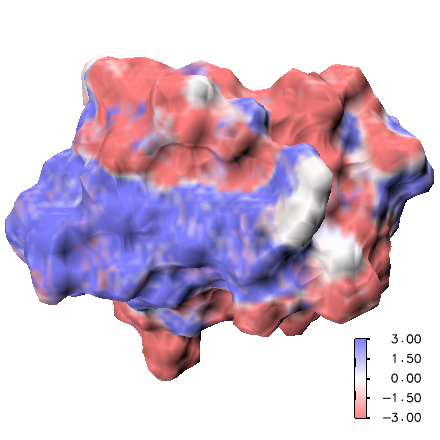
\includegraphics[width=2.1in]{1cbn_gfmlodie_back_scale_1.png}\\
  GFM-ADI back \hskip 0.7in GFM-LODCN back \hskip 0.7in GFM-LODIE back\\
	\caption{Electrostatic potential for 1cbn using $\Delta t = 0.05$ and $h= 0.5$. }
\label{fig_1cbn}
\end{center}
\end{figure}

%%%%%%%%%%%%%%%%%%%%%%%%%%%%%%%%%%%%%%%%%%%%%%%%%%%%%%%%%%%%%%%%%%%%%%%%%%%%%


\subsection{Solvation energy of 24 proteins}
Next we solve the nonlinear PBE and compute the solvation energy for a collection of 24 proteins as in \cite{Geng2007,Geng2017a}. The dielectric constants and Ionic strength are same as our study for the protein Crambin(1cbn) as $\epsilon^-=1, \epsilon^+=80$ and $I_s = 0.15$.
%The dielectric constants, Ionic strength and all other parameters have been set similar to our study for the protein Crambin(1cbn).  
 

\begin{table}[!ht]
\centering
\begin{tabular}{ c c c c c c c c}
\hline
\scriptsize{PDB} & \scriptsize{No. of Atoms}& \scriptsize{rMIB}   &   \scriptsize{ADI}    &  \scriptsize{GFM-ADI}  & \scriptsize{GFM-LODCN} & \scriptsize{GFM-LODIE}\\ \hline
1ajj & 519  & -1139.48 & -1371.10 & -1139.45 & -1139.07 & -1133.06 \\
2erl & 573  & -952.36  & -1165.28 & -952.13  & -951.03  & -945.96  \\
1cbn & 648  & -303.33  & -459.51  & -302.06  & -301.09  & -297.06  \\
1vii & 596  & -902.31  & -1154.67 & -901.78  & -901.36  & -895.15  \\
1fca & 729  & -1204.44 & -1458.16 & -1205.53 & -1205.09 & -1199.33 \\
1bbl & 576  & -988.40  & -1302.49 & -986.15  & -985.72  & -979.60  \\
2pde & 667  & -820.97  & -1018.66 & -819.17  & -819.83  & -813.45  \\
1sh1 & 702  & -753.99  & -999.92  & -751.69  & -751.84  & -745.15  \\
1vjw & 826  & -1241.07 & -1513.17 & -1244.74 & -1243.52 & -1236.67 \\
1uxc & 809  & -1139.25 & -1478.20 & -1138.50 & -1135.22 & -1128.39 \\
1ptq & 795  & -873.32  & -1170.00 & -867.98  & -867.40  & -859.71  \\
1bor & 832  & -853.47  & -1102.40 & -852.49  & -851.24  & -844.68  \\
1fxd & 824  & -3321.39 & -3653.81 & -3321.68 & -3321.34 & -3313.83 \\
1r69 & 997  & -1088.62 & -1419.35 & -1085.45 & -1084.66 & -1076.32 \\
1mbg & 903  & -1353.31 & -1685.70 & -1352.63 & -1351.30 & -1343.68 \\
1bpi & 898  & -1304.37 & -1672.02 & -1301.61 & -1299.86 & -1291.40 \\
1hpt & 858  & -812.49  & -1147.42 & -809.02  & -808.09  & -799.24  \\
451c & 1216 & -1027.21 & -1379.27 & -1023.71 & -1022.61 & -1012.70 \\
1svr & 1435 & -1711.11 & -2257.80 & -1707.87 & -1706.38 & -1693.11 \\
1frd & 1478 & -2862.50 & -3376.35 & -2863.69 & -2863.03 & -2850.42 \\
1a2s & 1272 & -1921.20 & -2292.15 & -1919.28 & -1917.70 & -1907.96 \\
1neq & 1187 & -1731.71 & -2223.08 & -1729.87 & -1728.61 & -1716.47 \\
1a63 & 2065 & -2374.41 & -3149.69 & -2370.80 & -2369.26 & -2350.42 \\
1a7m & 2809 & -2160.34 & -2771.41 & -2155.05 & -2152.48 & -2135.73 \\ \hline
\end{tabular}
\caption{Solvation energies ({\it kcal/mol}) of 24 Proteins considering $\Delta t = 0.001$ for ADI and $\Delta t =0.05$ for GFM-ADI, GFM-LODCN, GFM-LODIE. Stopping condition is set to be either $T_{end}=50$ or $\Delta E^n_{sol}<10^{-4}$.}  
\label{tab:24protein}
\end{table}


The solvation energies for all three of our proposed schemes are compared  with the rMIB and MIB schemes in Table \ref{tab:24protein} and Figure \ref{fig:24protein}(a). The results from our proposed schemes are very close to the results from the rMIB and MIB schemes while solving the nonlinear PBE instead of the linear PBE. As we have identified in the previous sections GFM-ADI method appeared to be more accurate than the other two of our proposed schemes and achieves the same level of accuracy as rMIB and MIB schemes. Table \ref{tab:24protein} also confirms that if the GFM-ADI method fails to converge for any protein then GFM-LODCN or GFM-LODIE can be used due to the fact that they are more stable and the results are not that much different than GFM-ADI.   

\begin{figure}[H]
	\begin{center}		
	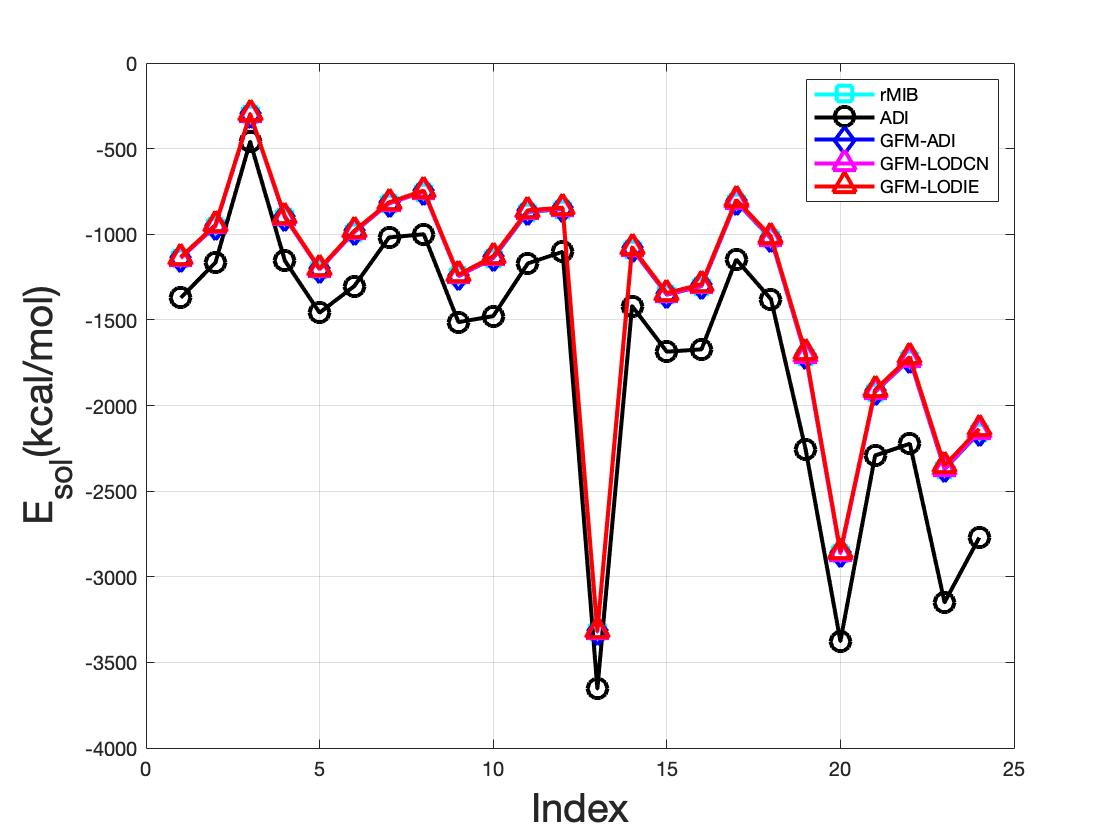
\includegraphics[width=\textwidth,height=270pt]{24_energy.jpg}\\
	(a)\\
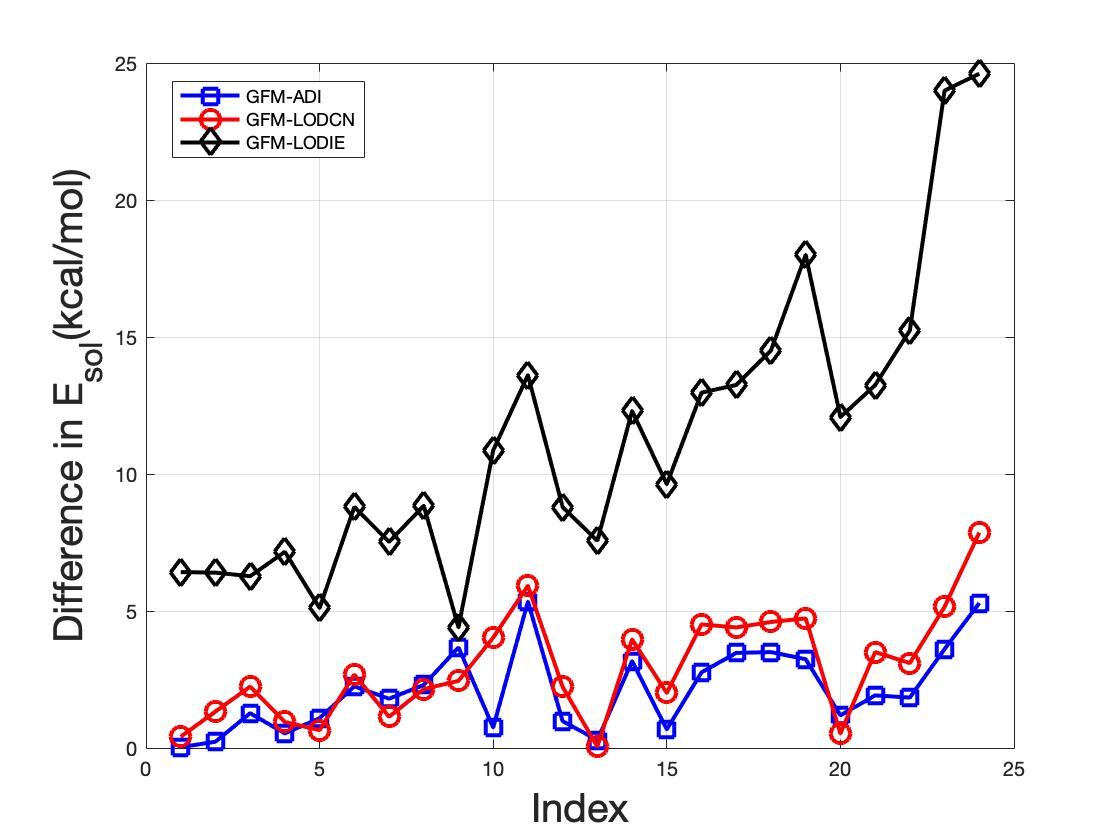
\includegraphics[width=\textwidth,height=270pt]{24_energy_diff.jpg}
	(b)\\ 
	\end{center}
\caption{(a) Solvation energy of 24 proteins. (b) Difference in Solvation energy compared to rMIB method. Here "Index" is the set of all 24 proteins indexed.}
\label{fig:24protein}
\end{figure}
It is noticeable in Figure \ref{fig:24protein} that the solvation energies for GFM-ADI, GFM-LODCN and GFM-LODIE are very close to each other. But the solvation energies from the ADI methods are always $200$ to $700$ $kcal/mol$ lower than the other proposed methods. This is an indicator that a major systematic difficulty like the singularity has been avoided to improve the accuracy in these newly proposed methods in this dissertation. We  also report the difference in the calculated solvation energy for our proposed methods with the rMIB method in Figure \ref{fig:24protein}. Figure \ref{fig:CPU_24protein} reports the required CPU time for these methods highlighting the fact that the ADI method takes around $10$ times more CPU time compared to the newly proposed methods. A major reason behind that is the necessity of $\Delta t$ to be as small as $0.001$ for the ADI method to keep it stable and accurate enough for all 24 proteins tested here. For the newly proposed methods we are able to use $\Delta t =0.05$ requiring less time to compute the solvation energies which are more accurate than the ADI method.    
\begin{figure}[H]
	\begin{center}
		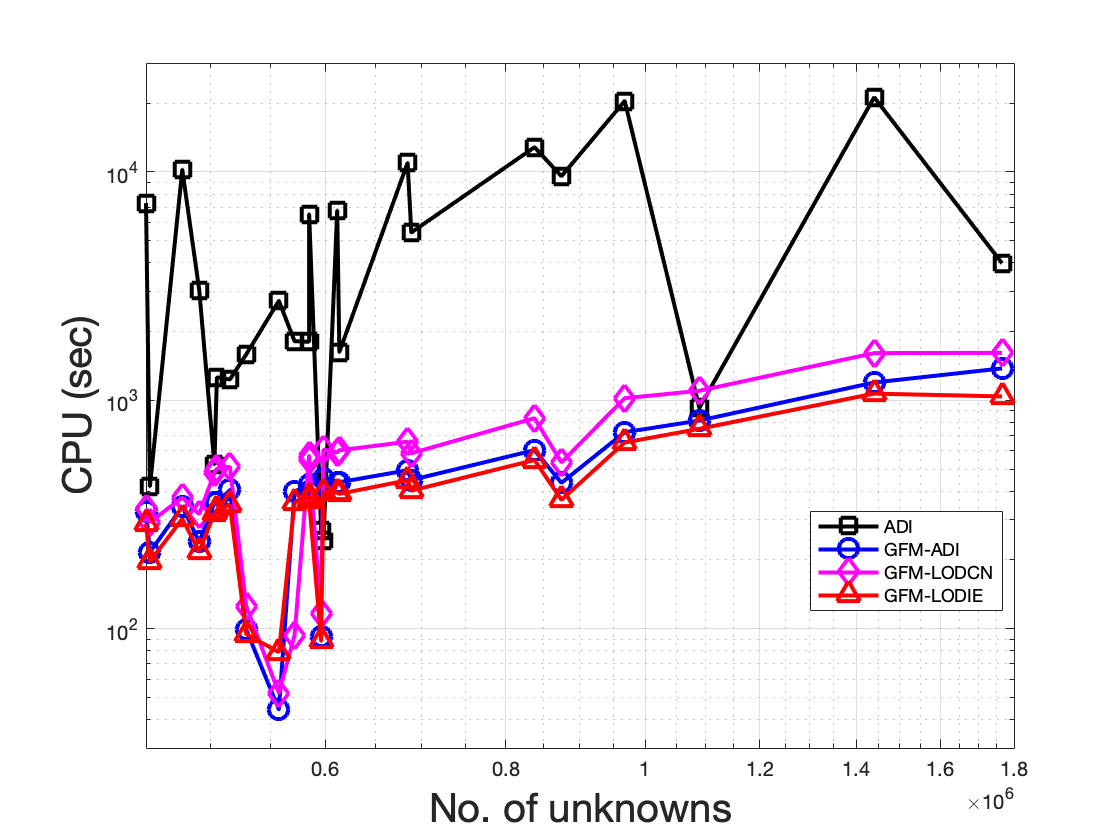
\includegraphics[width=\textwidth,height=300pt]{CPU_time.png}
	\end{center}
	\caption{CPU time for the Solvation Energy calculation of 24 proteins}
	\label{fig:CPU_24protein}
\end{figure}
%%%%%%%%%%%%%%%%%%%%%%%%%%%%%%%%%%%%%%%%%%%%%%%%%%%%%%%%%%%%%%%%%%%%%%%%%%%%%
\subsection{Binding energy of 2a9x}
Binding energies play an important role in viral transcription and antiviral drug design \cite{drug2}. In particular a better accuracy of the binding energy of the BIV Tat Protein and BIV TAR RNA in the HIV viral replication can significantly help in search of new antiviral drugs that repress the replication by blocking transactivation of viral RNA transcription \cite{Leeper2005}. In this section we demonstrate the ability of the GFM-ADI method to compute the binding energy of the BIV Tat Protein and BIV TAR RNA. 

\begin{table}[H]
\centering
\begin{tabular}{crrrr}
\hline
$h$ & $E_{\rm sol}^{\rm complex}$ & $E_{\rm sol}^{\rm protein}$ & $E_{\rm sol}^{\rm RNA}$ & $E_{\rm bind}^{\rm complex}$ \\ \hline
\multicolumn{5}{c}{rMIB}  \\ \hline
1   & -5816.38 & -1021.94 & -8893.39 & 383.60 \\
1/2 & -5821.22 & -1025.86 & -8898.54 & 387.84 \\
1/4 & -5823.39 & -1026.27 & -8900.52 & 388.05 \\ \hline
\multicolumn{5}{c}{GFM-ADI}  				  \\ \hline
1   & -5834.10 & -1027.14 & -8915.17 & 392.84 \\
1/2 & -5824.82 & -1025.98 & -8905.59 & 391.38 \\
1/4 & -5841.62 & -1026.40 & -8916.69 & 386.12 \\ \hline
\end{tabular}
\caption{Binding energy of 2a9x}
\label{tab_2a9x}
\end{table}

The electrostatic binding free energy can be calculated by the following formula based on the free energy cycle,
\begin{equation}
	E^{\rm AB}_{\rm bind}=\Delta G^{\rm AB}_{\rm ele}-\Delta G^{\rm A}_{\rm ele}-\Delta G^{\rm B}_{\rm ele}\label{eq_bind} =[E^{\rm AB}_{\rm sol}+E^{\rm AB}_{\rm cou}]-[E^{\rm A}_{\rm sol}+E^{\rm A}_{\rm cou}]-[E^{\rm B}_{\rm sol}+E^{\rm B}_{\rm cou}],
\end{equation}
where the free energies of the complex $AB$ and its monomers $A$ and $B$ on the RHS can be calculated from the solvation energies in equation (\ref{eq_Gele}). 

\begin{figure}[!ht]
	\begin{center}
		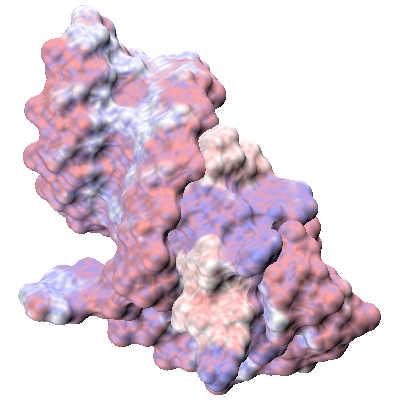
\includegraphics[width=3in]{complex_front.png}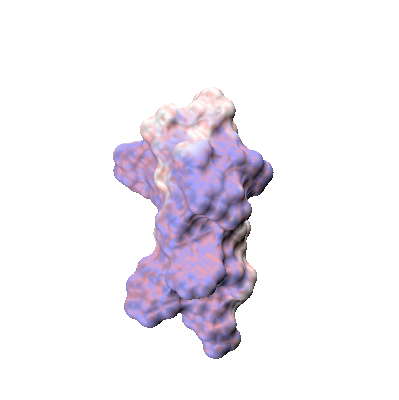
\includegraphics[width=3in]{protein_back.png}\\
		\hskip 0.5in 2a9x complex front\hskip 2.5in 2a9x  protein back\\
		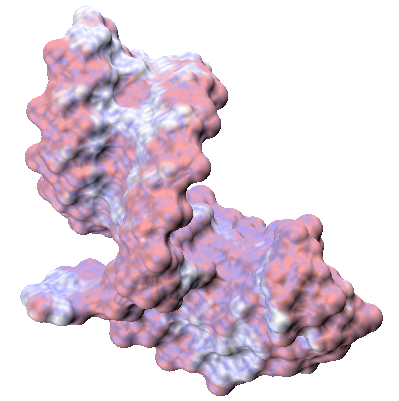
\includegraphics[width=3in]{rna_front.png}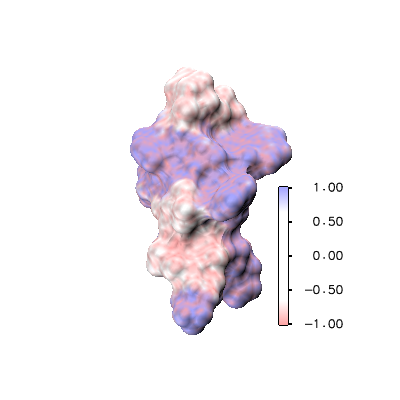
\includegraphics[width=3in]{protein_front_scale_right.png}\\
		\hskip 0.7in 2a9x rna front\hskip 2.8in 2a9x  protein front\\
		\caption{Electrostatic potential for 2a9x using GFM-ADI for $\Delta t = 0.05$ and $h = 0.5$}
		\label{fig:2a9x}
	\end{center}
\end{figure}


In Table \ref{tab_2a9x} we find that the binding energies calculated by GFM-ADI are very close to the results from rMIB method reported in \cite{Geng2017a}. This shows the ability of the GFM-ADI method to calculate other type of energies for large protein-ligand complexes like $2a9x$. In Figure \ref{fig:2a9x} the electrostatic potential of 2a9x and its monomers are visualized on their surface in a color scale. These type of visualizations help to provide optimized parameters for the molecular mechanics calculations of the drug candidate that will influence binding affinity \cite{drug2012}.      

%    where the calculated solvation energies ($E_{\rm sol}$) will be added with the coulomb energies ($E_{\rm cou}$) to get the free energies ($\Delta G$) for the complex $AB$ and the monomers $A$  and $B$. 


%%%%%%%%%%%%%%%%%%%%%%%%%%%%%%%%%%%%%%%%%%%%%%%%%%%%%%%%%%%%%%%%%%%%%%%%%%%%%

\subsection{Salt effect on the binding affinity}
The nonlinear PBE is often used to describe the salt effects on the binding of ligands, peptides, and proteins to nucleic acids, membranes, and proteins. In this investigation we have tested the performance of the proposed GFM-ADI scheme for the evaluation of the salt effect in the protein-protein binding of the complex Lactoglobulin dime(A-B) (PDB ID 1beb) and E9Dnase-Im9(10)(B-A)(PDB ID 1emv). Physically, the binding affinity can be quantitatively represented based on the binding-free energies, which reflect the non-specific salt dependence of the formation of macro- molecular complexes. The binding affinity is then calculated as the slope ratio of the salt-dependent binding energy at certain salt strength $I_s$ against the natural logarithm of $I_s$.
The electrostatic binding-free energy can be further split into $E_{\rm cou}(I_s)$'s as the salt-independent parts and $E_{\rm sol}(I_s)$'s as the salt-dependent parts. The variation of the salt-dependent part of the binding-free energy $\Delta E_{\rm bind}(I_s)$ can thus be calculated as the difference in $E_{\rm bind}(I_s)$ for some nonzero salt strength and the zero salt concentration, because the salt independent parts cancel out. Altogether we have the following formula:\\
\begin{eqnarray}
	\Delta E_{\rm bind}(I_s) &=& E_{\rm bind}(I_s)- E_{\rm bind}(0)\label{eq_del_e_bind} \nonumber\\
						 &=& [E_{\rm sol}^{\rm AB}(I_s)-E_{\rm sol}^{\rm AB}(0)]-[E_{\rm sol}^{\rm A}(I_s)-E_{\rm sol}^{\rm A}(0)]- [E_{\rm sol}^{\rm B}(I_s)-E_{\rm sol}^{\rm A}(0).
\end{eqnarray}
						 
\begin{figure}[!ht]
\begin{center}
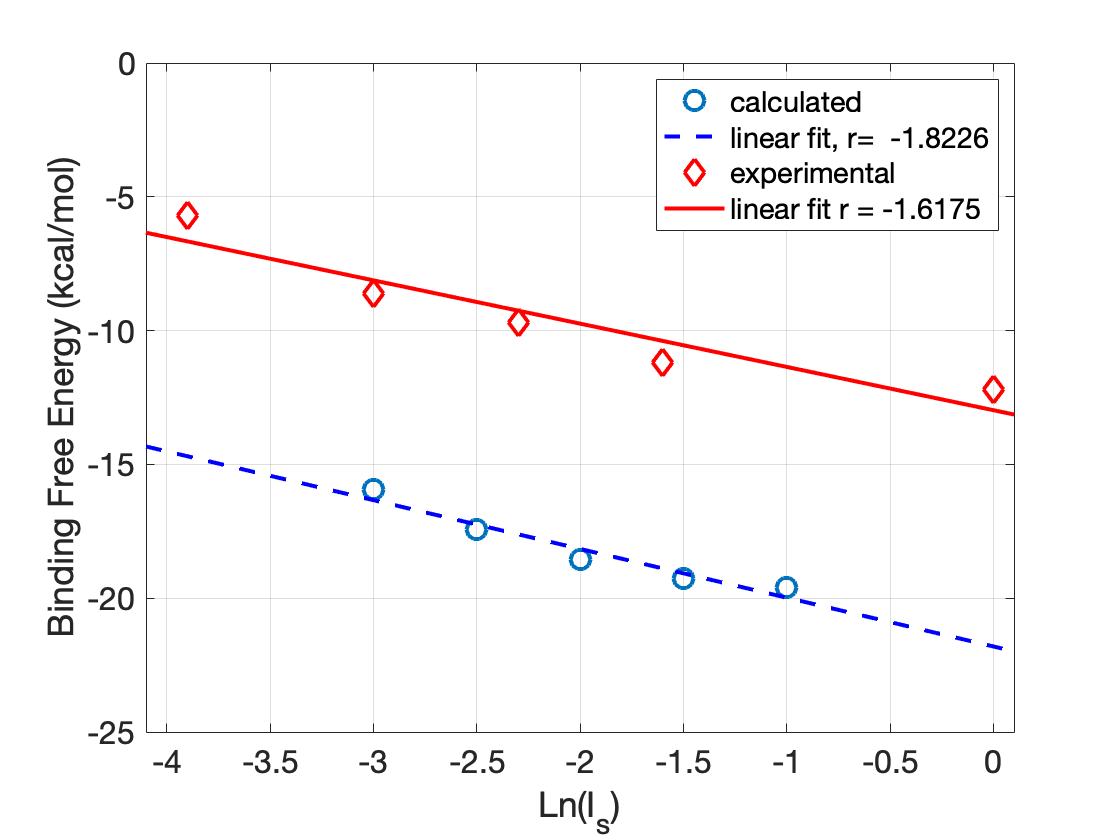
\includegraphics[width =3in]{1beb_Tend50_TTol_neg4}
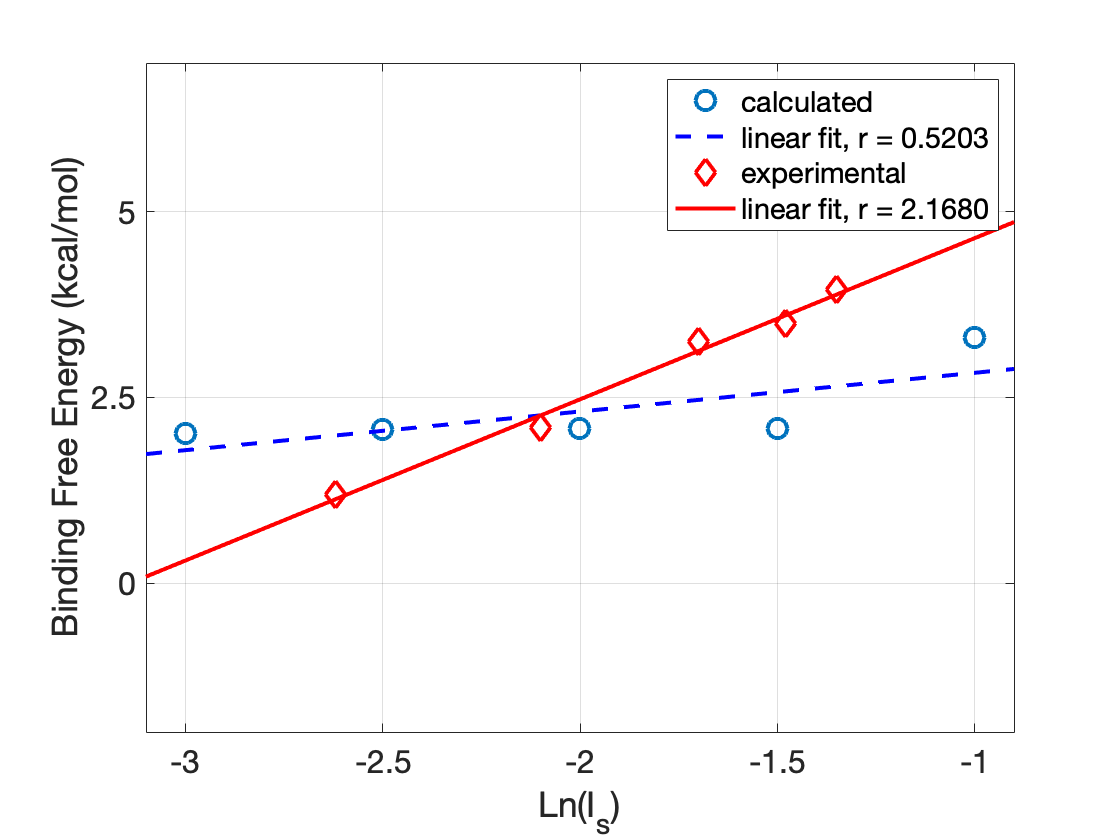
\includegraphics[width =3in]{1emv_Tend50_TTol_neg4}
\\
1beb \hskip 2.7in 1emv
\end{center}
\caption{The salt dependence of the binding affinities}
\label{fig_salt_effect}
\end{figure}

\begin{table}[!t]
\begin{center}
\begin{tabular}{ccclcrrr}
\hline
\multicolumn{1}{c}{}           & \multicolumn{3}{l}{Charges} & \multicolumn{3}{l}{Slope ratios} \\
 PDB  & AB    & A     & B      & Experimental & GFM-ADI & LFLPB   \\ \hline
 1beb & $+26$ & $+13$ & $+13$  & $-1.62$      & $-1.82$ & $-2.02$ \\ %\hline
 1emv & $-3$  & $-8$  & $+5$   & $2.17$       & $0.52$  & $2.4$   \\
 1brs & $-4$  & $+2$  & $-6$   & $0.96$		  &	$0.09$ & $0.67$ 	  \\
	 \hline
\end{tabular}
\caption{Comparison of binding affinities of the protein complexes}
\label{tab_salt_effect}
\end{center}
\end{table}

 
For this study we use the same model parameters as earlier for 24 proteins. In Figure \ref{fig_salt_effect} we report the calculated binding free energy with the experimental results. The slope ratio or the binding affinity is calculated and reported in Table (\ref{tab_salt_effect}) as in \cite{Zhao2011}. The results attained by the Lagrangian formulation linearized PB (LFLPB) model \cite{Zhan2011} are also given in Table (\ref{tab_salt_effect}) for comparison. For 1beb the binding affinity calculated by the GFM-ADI method is sufficiently close to experimental data and better than LFLPB. For $1emv$ and $1brs$ the results from the GFM-ADI method is not as good as those of the LFLPB model but qualitatively it agrees with the experimental observations; that is as the hetero-diemric complex, the binding-free energy increases when the ionic strength is larger. This is probably because the calculation of the binding affinity requires a physical cutoff to obtain two monomers A and B and the error in the mathematical modeling, i.e., the nonlinear Poisson Boltzmann electrostatic analysis is not enough for the calculation of the binding affinities. Other biophysical models have to be used in order to produce a better slope estimation. 
   	



